%%%%%%%%%%%%%%%%%%%%%%%%%%%%%%%%%%%%%%%%%%%%%%%%%%%%%%%%%%%%%%%%%%%%%%%%%%%%%%%
% TIME SCALE OF PHENOMENA IN ELECTRICAL SYSTEMS
%%%%%%%%%%%%%%%%%%%%%%%%%%%%%%%%%%%%%%%%%%%%%%%%%%%%%%%%%%%%%%%%%%%%%%%%%%%%%%%
\tikzstyle{caixa} = [rectangle, draw, thin, fill=white, text centered, rounded corners=2, minimum height=0.6cm, font=\footnotesize ] %,text width=2cm
\tikzstyle{vai} = [draw, rounded corners=1]
\tikzstyle{pontilhado} = [dotted, gray]
\tikzstyle{vaivolta} = [draw, thick, rounded corners=2, latex'-latex']
\tikzstyle{fonte} = [font=\footnotesize]
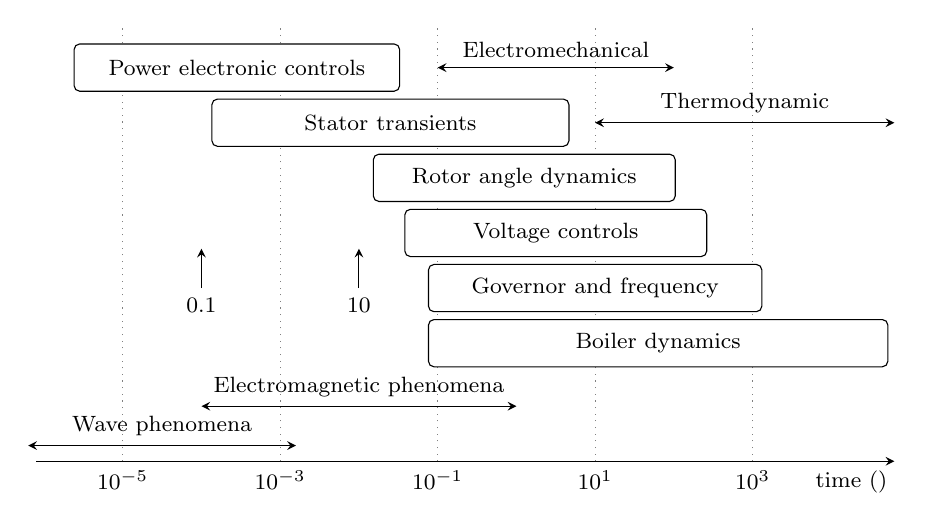
\begin{tikzpicture}[>=stealth]%[node distance=0.5cm]%, auto]
    %\draw [help lines] (-8,0) grid (5,-9);
    %-------------------------------------------------
    \draw [->,fonte] (-6.1,-0.5) -- node[pos=0.95,anchor=north] {time (\si{\second})} 	(4.8,-0.5);
    
    \foreach \x/\t in {-5/$10^{-5}$,-3/$10^{-3}$,-1/$10^{-1}$,1/$10^{1}$,3/$10^{3}$}
    {
    	\node at (\x,-0.5) [fonte, anchor=north] () {\t};	
    	\draw [pontilhado] (\x,-0.5) -- (\x,5);
    }
    
    \node at (1.8,1) [caixa,text width=5.6cm] () {Boiler dynamics};	
    \node at (1,1.7) [caixa,text width=4cm] () {Governor and frequency};	
    \node at (0.5,2.4) [caixa,text width=3.6cm] () {Voltage controls};	
    \node at (0.1,3.1) [caixa,text width=3.6cm] () {Rotor angle dynamics};	
    \node at (-1.6,3.8) [caixa,text width=4.3cm] () {Stator transients};	
    \node at (-3.55,4.5) [caixa,text width=3.9cm] () {Power electronic controls};	
    
    \draw [->,fonte] (-4,1.7) -- node[pos=0,anchor=north] {\SI{0.1}{\milli \second}} ++(0,0.5);
    \draw [->,fonte] (-2,1.7) -- node[pos=0,anchor=north] {\SI{10}{\milli \second}} ++(0,0.5);
    
    \draw [<->,fonte] (-4,0.2) -- node[above] {Electromagnetic phenomena}(0,0.2);
    \draw [<->,fonte] (-6.2,-0.3) -- node[above] {Wave phenomena}(-2.8,-0.3);
    \draw [<->,fonte] (-1,4.5) -- node[above] {Electromechanical}(2,4.5);
    \draw [<->,fonte] (1,3.8) -- node[above] {Thermodynamic}(4.8,3.8);
\end{tikzpicture}